\documentclass[border=10pt]{standalone}

\usepackage{tikz}
\usepackage{tikzsymbols}
\usetikzlibrary{calc,patterns,shapes.geometric}

\def\centerarc[#1](#2)(#3:#4:#5){\draw[#1] ($(#2)+({#5*cos(#3)},{#5*sin(#3)})$) arc (#3:#4:#5);}

\begin{document}
	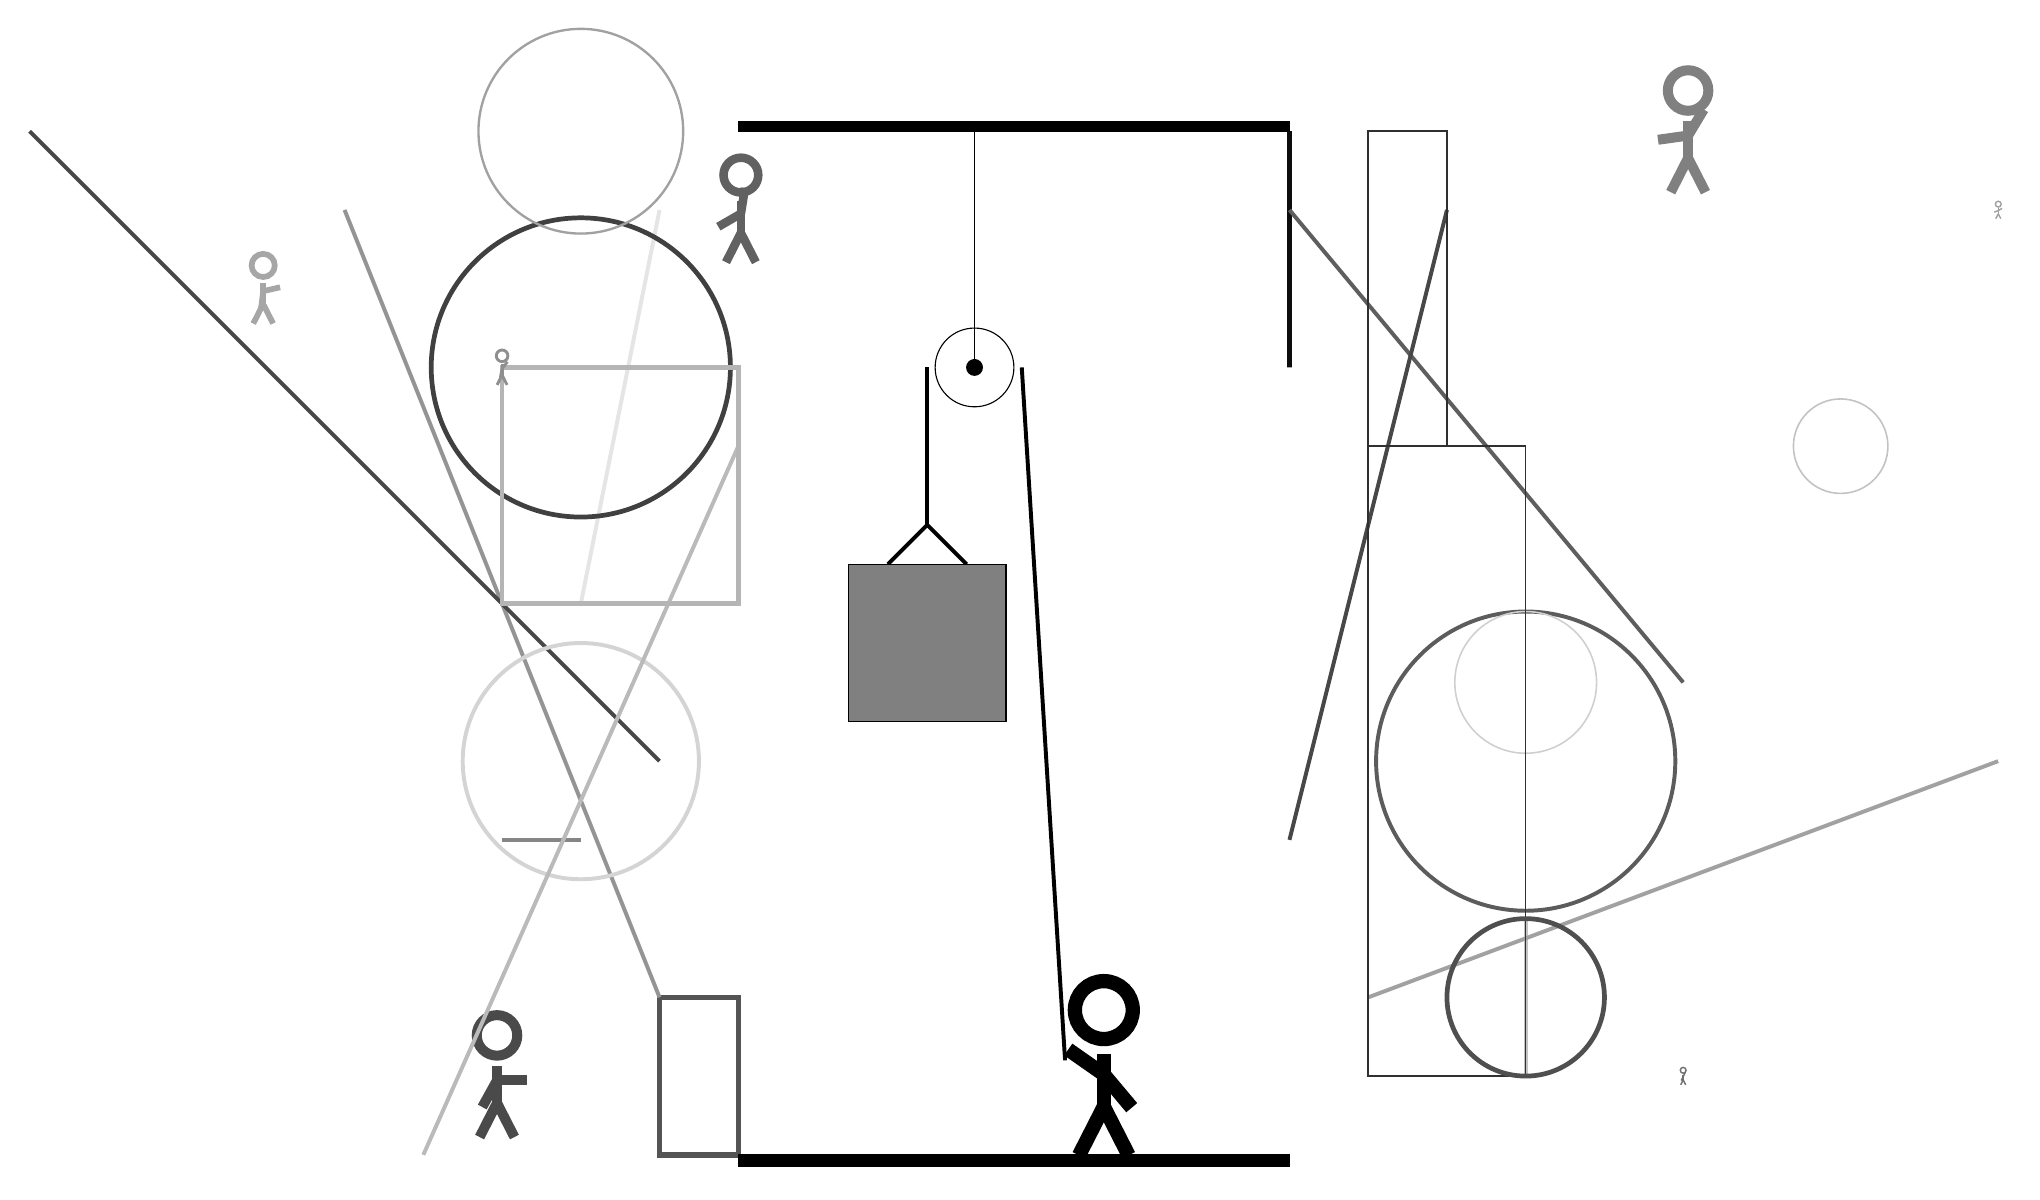
\begin{tikzpicture}
		%%%%% START %%%%%
		
		\draw[fill=black] (-2, 10) rectangle (5, 10.125);
		
		\draw[line width=0.7mm, color=black!67] (-2, -1) rectangle (-3, -3);
		
		\draw[line width=0.5mm, color=black!23](8, 0) -- (8, -2);
		\draw[line width=0.6mm, color=black!48] (-4, 1) rectangle (-5, 1);
		\draw[line width=0.7mm, color=black!95] (5, 7) rectangle (5, 10);
		\node[line width=0.5mm, color=black!56] at (10, -2) {\Strichmaxerl[1][62][64]};
		
		\node[line width=0.5mm, color=black!37] at (14, 9) {\Strichmaxerl[1][21][30]};
		\draw[line width=0.5mm, color=black!10](-4, 4) -- (-3, 9);
		\draw[line width=0.5mm, color=black!42](-7, 9) -- (-3, -1);
		\node[line width=0.4mm, color=black!50] at (10, 10) {\Strichmaxerl[7][8][59]};
		\draw [line width=0.6mm, color=black!75](-4, 7) circle (1.9);
		\draw[line width=0.5mm, color=black!37](6, -1) -- (14, 2);
		\draw[line width=0.5mm, color=black!63](10, 3) -- (5, 9);
		\draw[line width=0.5mm, color=black!72](5, 1) -- (7, 9);
		\draw[line width=0.5mm, color=black!72](-3, 2) -- (-11, 10);
		\draw [line width=0.5mm, color=black!64](8, 2) circle (1.9);
		\draw [line width=0.2mm, color=black!19](8, 3) circle (0.9);
		
		\draw[line width=0.2mm, color=black!81] (6, 6) rectangle (8, -2);
		\node[line width=0.6mm, color=black!71] at (-5, -2) {\Strichmaxerl[7][61][0]};
		\node[line width=0.2mm, color=black!35] at (-8, 8) {\Strichmaxerl[4][83][13]};
		\draw [line width=0.2mm, color=black!24](12, 6) circle (0.6);
		\draw [line width=0.3mm, color=black!37](-4, 10) circle (1.3);
		\draw [line width=0.5mm, color=black!17](-4, 2) circle (1.5);
		\node[line width=0.7mm, color=black!62] at (-2, 9) {\Strichmaxerl[6][30][81]};
		\draw [line width=0.6mm, color=black!69](8, -1) circle (1.0);
		\draw[line width=0.5mm, color=black!27](-2, 6) -- (-6, -3);
		\draw[line width=0.3mm, color=black!81] (6, 10) rectangle (7, 6);
		\draw[line width=0.6mm, color=black!29] (-2, 4) rectangle (-5, 7);
		\node[line width=0.4mm, color=black!44] at (-5, 7) {\Strichmaxerl[2][79][52]};
		
		\draw (1, 7) circle (0.5);
		\draw[fill=black] (1, 7) circle (0.1);
		\draw (1, 10) -- (1, 7);
		
		\draw[line width=0.5mm] (-0.1, 4.5) -- (0.4, 5.0) -- (0.9, 4.5);
		\draw[fill=black!50] (-0.6, 4.5) rectangle (1.4, 2.5);
		
		\draw[line width=0.5mm] (0.4, 7) -- (0.4, 5.0);
		\centerarc[line width=0.5mm](1, 7)(0:180:0.6);
		\draw[line width=0.5mm](1.6, 7) -- (2.15, -1.8);
		
		\node at (2.6, -1.9) {\Strichmaxerl[10][-35][-50]};
		
		\draw[fill=black] (-2, -3) rectangle (5, -3.15);
		
		%%%%% END %%%%%
	\end{tikzpicture}
\end{document}